%%%%%%%%%%%%%%%%%%%%%%%%%%%%%%%%%%%%%%%%%%%%%%%%%%%%%%%%%%%%%%%%%%%%%%%%%%%%%%%%
%2345678901234567890123456789012345678901234567890123456789012345678901234567890
%        1         2         3         4         5         6         7         8

\documentclass[letterpaper, 10 pt, conference]{ieeeconf}  % Comment this line out if you need a4paper



%\documentclass[a4paper, 10pt, conference]{ieeeconf}      % Use this line for a4 paper

\IEEEoverridecommandlockouts                              % This command is only needed if 
                                                          % you want to use the \thanks command

\overrideIEEEmargins                                      % Needed to meet printer requirements.

%In case you encounter the following error:
%Error 1010 The PDF file may be corrupt (unable to open PDF file) OR
%Error 1000 An error occurred while parsing a contents stream. Unable to analyze the PDF file.
%This is a known problem with pdfLaTeX conversion filter. The file cannot be opened with acrobat reader
%Please use one of the alternatives below to circumvent this error by uncommenting one or the other
%\pdfobjcompresslevel=0
%\pdfminorversion=4

% See the \addtolength command later in the file to balance the column lengths
% on the last page of the document

% The following packages can be found on http:\\www.ctan.org
%\usepackage{graphics} % for pdf, bitmapped graphics files
%\usepackage{epsfig} % for postscript graphics files
%\usepackage{mathptmx} % assumes new font selection scheme installed
%\usepackage{times} % assumes new font selection scheme installed
\usepackage{amsmath} % assumes amsmath package installed
\usepackage{amssymb}  % assumes amsmath package installed
\usepackage{hyperref}


 \usepackage{easyReview}
 


\title{\LARGE \bf
Matrix Multiplication-Driven Repulsive Fields for 3D Voxel-Based TSDF Calculation
}


\author{
	Jakob Baumgartner$^{1}$ and Gregor Klančar$^{2}$% <-this % stops a space
%\thanks{*This work was not supported by any organization}% <-this % stops a space
%\thanks{$^{1}$Albert Author is with Faculty of Electrical Engineering, Mathematics and Computer Science,
%        University of Twente, 7500 AE Enschede, The Netherlands
%        {\tt\small albert.author@papercept.net}}%
%\thanks{$^{2}$Bernard D. Researcheris with the Department of Electrical Engineering, Wright State University,
%        Dayton, OH 45435, USA
%        {\tt\small b.d.researcher@ieee.org}}%
}


\begin{document}



\maketitle
\thispagestyle{empty}
\pagestyle{empty}


%%%%%%%%%%%%%%%%%%%%%%%%%%%%%%%%%%%%%%%%%%%%%%%%%%%%%%%%%%%%%%%%%%%%%%%%%%%%%%%%
\begin{abstract}



\end{abstract}


%%%%%%%%%%%%%%%%%%%%%%%%%%%%%%%%%%%%%%%%%%%%%%%%%%%%%%%%%%%%%%%%%%%%%%%%%%%%%%%%
\section{INTRODUCTION}

\section{RELATED WORKS}

\section{REPULSIVE FIELD CALCULATION}

The robots environment is modelled by discrete voxels. As the robots environment can dynamically change, we propose a method that looks at the surrounding space of the robot and calculates these direction away from all the surrounding obstacles in real time. We only look in a predefined area / perimeter arround the robot.  

In 3D computer graphics, a voxel represents a value on a regular grid in three-dimensional space. Each of the voxels holds the probability value of its occupation. In case of voxel being empty it holds the value of 0, if the voxel is occupied it holds the value of non-zero, depending on our assurance of it being occupied. If it is definitly occupied it holds the value of 1. 

Mreža voxels je lahko predefinirana, glede na model / 3d zemljevid prostora. Zasedenost voxlov lahko spreminjamo glede na poznane pozicije in trajektorije preostalih agentov v prostoru. Kot omenjeno v uvodu, pa lahko zasedenost voxlov pridobimo tudi z senzorskimi sistemi. 

In our method, we compute repulsive velocities within the task space using a novel matrix kernel multiplication approach. Concentrating on the task space is advantageous as it provides a more direct and realistic representation of the environment. 

\replace{Naša metoda je posebno primerna za uporabo z senzorskimi sistemi kot so LIDAR ali globinske kamere, saj zaradi upoštevanja celotne okolice točke in ne le razdalje do najbližje točke v okolici efektivno filtriramo senzorski šum.}{prestavi to v diskusijo}

Repulsive velocities tell the agent in which direction to move, so that it avoids nearby obstacles. These velocities drop to zero when the agent maintains a minimum safe distance from obstacles, and rise to their highest when it nears an obstacle, facilitating immediate evasive action. As the repulsive field calculation is locally based, it will also go to zero when the agent is surrounded by all directions, equally spaced from all sides. That is, it is in the best local minima away from all the obstacles. 

\subsection{MAPPING}

Since the obstacle space is discrete (has finite resolution), while the Cartesian space is continuous, we propose two methods for mapping from Cartesian space to the occupancy grid space. The simpler approach involves mapping the point directly to the center of the nearest occupancy grid voxel, based on Euclidean distance.\add{is this clear, do i need equation?} However, this discretization can sometimes lead to discontinuities. Therefore, we propose a second approach: tri-linear interpolation of the calculated repulsive field to achieve a continuous repulsive field value.

Once the mapping of these points to the voxel grid is completed, we proceed to employ a specialized kernel convolution method. This method is tailored to calculate the components of the avoidance velocity vector in the Cartesian space, we generate the corresponding kernel and extract a segment of the obstacle grid of matching size, centered at agent or the point of interest (POI), resulting in two same size 3D matrices—one is a "window" from the obstacle grid $A_d$ and the other representing the kernel $K_d$.

If the agent is located near the edge of our known voxel grid we can set the eleemnts of the window would be located in the space beyond the matrix as empty in which case the robot might want to move towards this space or as occupied, which will prevent the robot from moving out of the known grid space.

By employing the Hadamard (element-wise) product (eq.~\ref{eq:hadamard}) between the cutout segment of the obstacle grid \(G_d\) and the corresponding 3D convolutional kernel \(W_d\) and than summoning all of the matrix values for each of the directions $d \in \{x, y, z\}$, we derive the resultant repulsive velocities vector \( \vec{v}_i = \left[ v_{x_i} v_{y_i} v_{z_i}\right] \).

%\begin{equation}
%	C_d = A_d \odot K_d
%	\label{eq:hadamard}
%\end{equation}

\begin{equation}
	v_d = \sum_{i,j,k} (G \odot W)_{ijk} = \sum_{i}\sum_{j}\sum_{k} g_{\Delta i \Delta j \Delta k} ~  w_{\Delta i \Delta j \Delta k}
\end{equation}


%\begin{equation}
%	\dot{x}_{poi} = \sum_{i}\sum_{j}\sum_{k} c_{dijk} 
%	\label{eq:summation}
%\end{equation}
%
%\alert{remove the above equation and add a vector of calculated velocities equation instead}
%
%\comment{}{TODO: add the indexes for x,y,z directions}



\subsection{KERNELS SELECTION}

The fundamental concept of our directional kernels lies in computing the repulsive field individually for each direction within the Cartesian coordinate system. \remove{Our filters structure was inspired by the Sobel  operator, a 2D convolutional filter frequently utilized in computer vision for calculating image gradients at specific points.}

Our kernels are designed as three-dimensional matrixes with a primary kernel axis aligned along a specific Cartesian direction, corresponding to the calculated repulsive velocity. The two secondary kernel axes are orthogonal to this primary axis. The distribution of values along the primary axis is inversely symmetric, exhibiting positive values on one side and negative values on the other, with the zero valued cell in the center of the kernel, where jump between max positive and max negative magnitude is. The function of the increase in magnitude along the primary axis of the kernel defines the shape of the repulsive velocity field, determining how the repulsive velocity changes as the agent approaches an obstacle. Moreover, it is essential for the magnitudes at the kernel's periphery to be minimal, promoting a smooth increase in repulsive velocity when approaching the obstacle rather than a sudden spike.

% KERNEL WEIGHTS

% PRIMARY AXIS

We propose two different primary axis weights distributions, of course there is no reason why any other distribution of weights could not be used. The choice of the weights distribution should depend on the profile of the repulsive velocities we want to archieve for the APF. 

The first of the proposed functions is a mirrored normal / gaussian distribution. By changing the sigma we can control how fast or slow does the field value grow when we approach obstacles.

$\Delta i = c_i - i$, $\Delta j = c_j - j$ in $\Delta k = c_k - k$ predstavljajo število celic odmika od centralnega polja matrike, v katerem se nahaja naša točka na agentu v posamezno koordinatno smer.

\begin{equation}
w_{\Delta i} = 
\begin{cases} 
	e^{-\frac{\Delta i^2}{2\sigma^2}} / (\sigma \sqrt{2\pi}) & \text{if } \Delta i > 0 \\
	0 & \text{if } \Delta i = 0 \\
	-e^{-\frac{\Delta i^2}{2\sigma^2}} / (\sigma \sqrt{2\pi}) & \text{if } \Delta i < 0 
\end{cases}
\end{equation}

%\begin{equation}
%w_i = 
%\begin{cases} 
%	\frac{e^{-\frac{\Delta i^2}{2\sigma^2}}}{\sigma \sqrt{2\pi}} & \text{if } \Delta i > 0 \\
%	0 & \text{if } \Delta i = 0 \\
%	-\frac{e^{-\frac{\Delta i^2}{2\sigma^2}}}{\sigma \sqrt{2\pi}} & \text{if } \Delta i < 0 
%\end{cases}
%\end{equation}

Another distribution we used is mirrored linear, where the $l=\lfloor width / 2 \rfloor$ is the rounded down half length of the primary axis kernel. 

\begin{equation}
	w_{\Delta i} = 
	\begin{cases} 
	 	\frac{l - \Delta i}{l} & \text{if } \Delta i > 0 \\
		0 & \text{if } \Delta i = 0 \\
		\frac{l + \Delta i}{l}& \text{if } \Delta i < 0 
	\end{cases}
\end{equation}

% ORTHAGONAL AXIS

If the matrix would be only 1 field width and height the field would work kind of as ray tracing in each of the main cartesian coordinate directions. Since our need is to detect also obstacles that dont align perfectly along the cartesian direction, it is important that our matrixes have width and height. However as we want bigger repulsive field when the obstacle is head on in the direction than when the obstacle is off the cardinal direction, we propose the following multiplicator, to account for the off direction obstacles.




The length of the primary axis is critical, as it dictates the detection range for obstacles. Longer kernels can detect obstacles further away
from the robot, essentially extending the ’safety zone’ around the robot. If the primary axis is too long, it can lead to extra calculations and may cause the robot to unnecessarily avoid obstacles that aren't in its immediate path, making its movement and path planning less efficient. A kernel with a primary axis that is too short might restrict the robot's ability to maneuver, detecting obstacles potentially too late, compromising the robots capacity to avoid obstacles effectively (eq. \ref{eq: detect range}). 

\begin{equation}
	\label{eq: detect range}
	num_{primary} = \frac{2 \times \mathrm{range}}{\Delta \mathrm{grid}}\\
\end{equation}

\add{mogoče dodaj še kak stavek o izbiri dimenzij matrik}

%\remove{In the orthogonal axes, the magnitude of values diminishes with increasing distance from the core of the kernel, nearing zero at the edges. This gradation is vital for a smooth velocity transition when obstacles emerge in the kernels range. The peak magnitude is located at the kernel's core, along the primary axis. The polarity of the values is determined by their position relative to the primary axis. }

The length of the orthogonal axes influences the peripheral detection range for obstacles. Excessively wide kernels may generate repulsive velocities for objects that are not in the path of the robot, whereas too narrow kernels might only detect obstacles aligned directly with the Cartesian direction in the point of interest. When selecting the width and height of the kernel, we must consider the density of the neighboring points of interest on the agent, ensuring that the \replace{collective fields}{combination of kernels} adequately cover the entire agent's surrounding area. 

For smooth transitions when approaching the obstacles we propose the following sinus based function for the orthagonal axis distributions. The proposed equation is the same for both of the orthagonal matrix directions / axis. That is of course while operating with axis the $r=\lfloor width / 2 \rfloor$ is the rounded down half length of the selected orthagonal axis kernel.

\begin{equation}
	w_{\Delta j} =
	\begin{cases} 
		sin(\left| \Delta j \right| \pi / (2 r)) & \text{if } \Delta j < 0 \text{~or }  \Delta j > 0 \\
		1 & \text{if } \Delta j = 0 \\
	\end{cases}
\end{equation}

Another option is to use linearly falling weights.

\begin{equation}
	w_{\Delta j} =
	\begin{cases} 
		\frac{l - \Delta j }{l} & \text{if } \Delta j < 0 \text{~or }  \Delta j > 0 \\
		1 & \text{if } \Delta j = 0 \\
	\end{cases}
\end{equation}


Finally we get three matrix kernels, one for each of the three coordinate axis directions by multiplieing weights components for primary and orthagonal axis.

\begin{equation}
	w_{\Delta i \Delta j \Delta k} = w_{\Delta i} * w_{\Delta j} * w_{\Delta k}
\end{equation}

Če imamo opravka s točkastim agentom, kot je recimo štirikopet - dron, potem je dobra oblika posameznih matrik enaka dimenzija dolžine, širine in višine. Tako dobimo enakomerno pokritost krogle prostora v okolici agenta in preprečimo mrtve kote, ki se sicer lahko pojavijo, ko se ovira nahaja v bližini agenta, vendar med posameznimi jedri. \add{ADD:primer,slika}

\comment{}{PLOT: kernel 2D images}

\subsection{3D INTERPOLATION} 


It is essential that the velocity contributions affecting the robot change smoothly. However, since our obstacle grid is discretely defined, achieving perfect continuity can be challenging. Increasing the resolution of the obstacle field can theoretically bring us closer to continuous behavior, but in practice, we are constrained by finite resolution. To ensure that the velocity remains continuous when transitioning from one cell of the obstacle grid to another at a point of interest (POI), we employ trilinear interpolation. \remove{This technique allows for a smooth and continuous linear approximation of velocities in all three Cartesian directions (x, y, and z) as the POI moves between cells.}

We start by scalling the coordinates of POI into the grid koordinate system, by multiplying it by grid resolution (eq.~\ref{eq:scale grid}). 

\begin{equation}
	\label{eq:scale grid}
	\vec{P} = \vec{p}_{\mathrm{POI}} \times\Delta \mathrm{grid}
\end{equation}

We get the indexes of the surrounding cells by first scaling the POI position by grid resolution and than rounding the position to the nearest lower and upper integer positions (eq.~\ref{eq:floor and ceil}).

%\begin{equation}
% X = \left[ \lfloor p_{x} \rfloor, \lceil p_{x} \rceil \right] 
%\end{equation}
%
%\begin{equation}
% Y = \left[ \lfloor p_{y} \rfloor, \lceil p_{y} \rceil \right] 
%\end{equation}
%
% \begin{equation}
% Z = \left[ \lfloor p_{z} \rfloor, \lceil p_{z} \rceil \right] 
%\end{equation}

\begin{equation}
	\label{eq:floor and ceil}
	\vec{P} =
	\begin{bmatrix}
		X \\
		Y \\
		Z \\
	\end{bmatrix}
	=
	\begin{bmatrix}
		\; \lfloor \vec{p}_{\mathrm{POI}}(1) \rfloor \; \lceil \vec{p}_{\mathrm{POI}}(1) \rceil \;  \\
		\; \lfloor \vec{p}_{\mathrm{POI}}(2) \rfloor \; \lceil \vec{p}_{\mathrm{POI}}(2) \rceil \; \\
		\; \lfloor \vec{p}_{\mathrm{POI}}(3) \rfloor \; \lceil \vec{p}_{\mathrm{POI}}(3) \rceil \; 
	\end{bmatrix}
\end{equation}

Once we got the indexes of the eight surrounding cells of our POI, we use our kernel matrix multiplication method, to calculate the 3x1 repulsive velocity vectors for all the cells (eq.~\ref{eq: calc rep vel}).

\begin{equation}
	\label{eq: calc rep vel}
	\vec{V}rep_{xyz,ijk} = \mathrm{calc\_rep\_vel}(X[i], Y[j], Z[k]) \quad \forall i, j, k \in \{1, 2\}
\end{equation}

Trilinear interpolation method works on a 3-dimensional regular grid. Before we can start with the interpolation we need to calculate the distance between POI and smaller coordinates of the cells where we calculated the repulsive velocities (eq.~\ref{eq: deltas interp}). \replace{Since the repulsive values we calculate for the cells are alligned with the centers of the cells, we need to move before the interpolation the positions of known grid points by half of the cell width.}{The calculated repulsive velocity values are located at the centers of the cells. Therefore, before interpolation, we shift the values of the cells coordinates by half the resolution of the obstacle grid for each direction. }

%\begin{equation}
%	\Delta X = \frac{\left( P_x - \left( X(1) + \frac{1}{2} \Delta \mathrm{grid} \right)  \right)}{\left( X(2) - X(1) \right)}
%\end{equation}
%
%\begin{equation}
%	\Delta Y = \frac{\left( P_y - \left( Y(1) + \frac{1}{2} \Delta \mathrm{grid} \right)  \right)}{\left( Y(2) - Y(1) \right)}
%\end{equation}
%
%\begin{equation}
%	\Delta Z = \frac{\left( P_z - \left( Z(1) + \frac{1}{2} \Delta \mathrm{grid} \right)  \right)}{\left( Z(2) - Z(1) \right)}
%\end{equation}

\begin{equation}
	\label{eq: deltas interp}
	\Delta \vec{P} =
	\begin{bmatrix}
		\Delta x \\
		\Delta y \\
		\Delta z		
	\end{bmatrix}
	=
	\begin{bmatrix}
		\frac{\left( P_x - \left( X(1) + \frac{1}{2} \Delta \mathrm{grid} \right)  \right)}{\left( X(2) - X(1) \right)} \\
		\frac{\left( P_y - \left( Y(1) + \frac{1}{2} \Delta \mathrm{grid} \right)  \right)}{\left( Y(2) - Y(1) \right)} \\
		\frac{\left( P_z - \left( Z(1) + \frac{1}{2} \Delta \mathrm{grid} \right)  \right)}{\left( Z(2) - Z(1) \right)} \\
	\end{bmatrix}
\end{equation}

The result of the interpolation is independent of the order of the operations. We first interpolate along the x-axis, followed by along the y-axis and finally along z-axis.

%\begin{equation}
%	\vec{V}_{rep,00} = \vec{V}_{rep,000}(1 - x_d) + \vec{V}_{rep,100}x_d
%\end{equation}
%\begin{equation}
%	\vec{V}_{rep,01} = \vec{V}_{rep,001}(1 - x_d) + \vec{V}_{rep,101}x_d
%\end{equation}
%\begin{equation}
%	\vec{V}_{rep,10} = \vec{V}_{rep,010}(1 - x_d) + \vec{V}_{rep,110}x_d
%\end{equation}
%\begin{equation}
%	\vec{V}_{rep,11} = \vec{V}_{rep,011}(1 - x_d) + \vec{V}_{rep,111}x_d
%\end{equation}
	
\begin{equation}
	\label{eq: interp x}
	\vec{V}rep_{xyz,jk} = \vec{V}rep_{xyz,0jk}(1 - \Delta x) + \vec{V}rep_{xyz,1jk} \, \Delta x \quad \forall \, j, k \in \{1, 2\}
\end{equation}

%\begin{equation}
%	\vec{V}rep_{xyz,0} = \vec{V}rep_{xyz,00}(1 - \Delta y) + \vec{V}rep_{xyz,10} \, \Delta y
%\end{equation}
%
%\begin{equation}
%	\vec{V}rep_{xyz,1} = \vec{V}rep_{xyz,01}(1 - \Delta y) + \vec{V}rep_{xyz,11} \, \Delta y
%\end{equation}

\begin{equation}
	\label{eq: interp y}
	\vec{V}rep_{xyz,k} = \vec{V}rep_{xyz,0k}(1 - \Delta y) + \vec{V}rep_{xyz,1k} \, \Delta y \quad \forall \, k \in \{1, 2\}
\end{equation}

\begin{equation}
	\label{eq: interp z}
	\vec{V}rep_{xyz} = \vec{V}rep_{xyz,0}(1 - \Delta z) + \vec{V}rep_{xyz,1} \, \Delta z 
\end{equation}

The final result is a repulsive velocity vector that transitions smoothly between the discrete values calculated at distinct points in the obstacle grid.

\begin{figure}
	\centering
	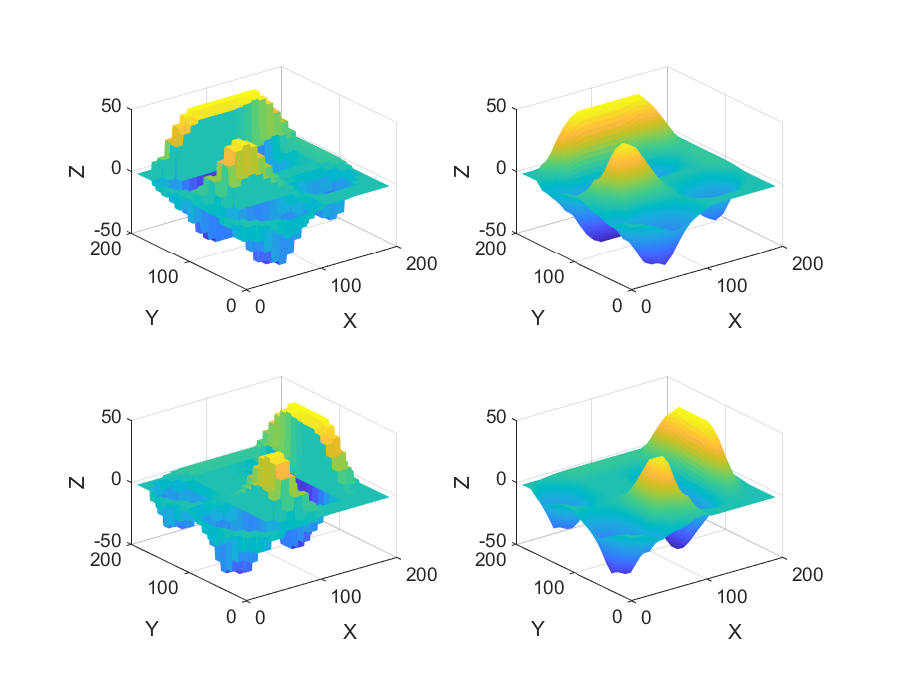
\includegraphics[width=1\linewidth]{non_and_interp_4_plots.eps} % Replace 'example-image' with the filename of your image
	\caption{Repulsive field generation via convolutional kernels. Left: Original repulsive fields in X (top) and Y (bottom) directions. Right: Corresponding fields using interpolation, showcasing enhanced smoothness.}
	\label{fig:interp-experiment}
\end{figure}

\section{MANIPULATOR KINEMATICS}

\subsection{INVERSE KINEMATIC CONTROL}

The desired movement of the end-effector is achieved by using inverse kinematics velocity control scheme with task prioritisation. 

\begin{equation}
	\dot{q} = J^+ \xi_{p} \mathrm{\vec{v}_{att}} + \dot{q}_{rep}
\end{equation}

The damped Moore-Penrose pseudo-inverse, \(J^+~=~J'(JJ' + \sigma_{ee} I)^{-1}\), is utilized to mitigate singularity issues and improve numerical stability in inverse kinematics computations. $\xi_{p}$ is the primary task execution slowdown constant. Finally $\dot{q}_{REP}$ are the weighted sum of avoidance joint velocities, each transformed into the null space of primary velocities, as described in the chapter below. \remove{For redundant robots, it optimizes solution selection by minimizing the joint velocity norm, while damping is applied to limit excessive joint velocities near singular configurations, thus improving solution robustness.}

\add{maybe add the middle joints component in the equation (it is not necessary, doesn't make much change in the chosen experiments)}

We run the inverse kinematics algorithm once for every time step, until we reach the desired cost function or reach the selected time limit. 

\subsection{END-EFFECTOR VELOCITY}

Vodenje vrha manipulatorja (end-effector) je naloga z najvišjo prioriteto. 

\remove{Our method employs inverse kinematics approach (IK) to guide the end effector (EE) towards its target, marking a departure from Khatib's joint coordinates approach in favor of a Cartesian coordinates framework. This is particularly beneficial in scenarios involving redundant manipulators, where determining an optimal goal joint configuration in advance is challenging.}

When calculating translational velocity, we avoid the conventional gradient of the squared distance approach, which leads to high initial velocities and subsequently slow speeds near the target. Our aim is a consistent velocity throughout the trajectory, with controlled deceleration near the goal. This is achieved by first calculating the unit vector towards the target for direction, then modulating its magnitude using a sigmoid function, specifically the arctangent function, to prevent overshooting and ensure stable approaching motion.

\begin{equation} 
	\vec{v} = \frac{\vec{x}_{EE} - \vec{x}_g}{||\vec{x}_{EE} - \vec{x}_g||} \times \frac{\arctan(k_{sigm} \; ||\vec{x}_{EE} - \vec{x}_g||) }{pi/2}
	\label{eq: v_att}
\end{equation}

In the above equation (eq.~\ref{eq: v_att}), $\vec{v}$  represents the end effector's translational velocity towards the target, combining direction and magnitude. The terms $\vec{x}_{EE}$ and $\vec{x}_g$ denote the current and goal positions of the EE, respectively, in Cartesian coordinates. The unit vector calculation, $\frac{\vec{x}_{EE}-\vec{x}_g}{||\vec{x}_{EE}-\vec{x}_g||}$, ensures motion directed towards the target. Finally, the sigmoid function, particularly the arctangent component, modulates this velocity to avoid overshooting, balancing speed and precision. The constant $k_{sigm}$ allows us to set how close to the goal does the robot EE start slowing down.

The rotational velocity error of the EE is needed for ensuring goal orientation of the EE. In our approach, orientations are depicted using rotation matrices. Specifically, \( R \) represents the current EE orientation, while \( gR \) signifies the goal EE orientation. The disparity between these orientations is encapsulated by the relative rotation matrix \( dR \). This matrix is formulated by multiplying the goal orientation matrix \( gR \) with the transpose of the current orientation matrix \( cR^{T} \). To ensure that it represents a pure rotation without any scaling we than normalize the so gotten matrix .

\begin{equation}
	dR = \frac{gR \cdot cR^{T}}{||gR \cdot cR^{T}||}
	\label{eq: rot_diff_mat}
\end{equation}

The relative rotation matrix value is converted into a quaternion, which is then logarithmically transformed \remove{to represent the rotational error vectorially}. The components of this quaternion, excluding the real part, than form the rotational error vector \( \omega \).

\begin{equation}
	dR \mapsto dQ = a + b \, i + c \, j + d \, k
	\label{eq: quat_mapsto}
\end{equation}

\begin{equation}
	dQl = 2 \cdot \log(dQ) = al + bl \, i + cl \, j + dl \, k
	\label{eq:quat_log}
\end{equation}

\alert{There needs to be an explanation why log, where is this from. Maybe a reference. cite: DMP Quaternions article Petrič, Žlajpah, Ude}



\begin{equation}
	\vec{\omega} =
	\begin{bmatrix}
		bl \\
		cl \\
		dl
	\end{bmatrix}
	\label{eq:rot_error_vector}
\end{equation}

To get the full velocity of the end effector (EE), \( \mathrm{\vec{v}_{ATT}} \), we combines translational and rotational velocities, which we scale using proportional gains \( k_p \) and \( k_r \).

\begin{equation}
	\mathrm{\vec{v}_{att}} = 
	\begin{bmatrix}
		k_pv* \vec{v}   \\
		k_{\omega} * \vec{\omega}
	\end{bmatrix}
	\label{eq:ee_velocity}
\end{equation}

Ker uporabljamo preslikavo v ničelni prostor primarne hitrosti (null space), lahko v primeru velikih hitrosti primarne naloge preostane premalo prostostnih stopenj, da bi se lahko varno izognili oviram. 

\label{chap:primary slowdown}

To ensure the primary task doesn't overpower the secondary task, we've integrated a primary task execution slowdown. This mechanism can reduce the manipulator's velocity towards its primary goal, leaving more maneuverability space for the secondary tasks.

\begin{equation}
	\label{eq:slowdown}
	\xi_{p}=
	\frac{1}{1 + \kappa_{\text{sec}} \delta_{min}}
\end{equation}

The slowdown factor (eq.~\ref{eq:slowdown}) is influenced by the constant \( \kappa_{\text{sec}} \) and the robot's minimum distance from an obstacle \( \delta_{\text{min}} \). We calculate the minimal distance in the repulsive velocities phase of the algorithm, as explained in section~\ref{chap:repulsive velocity}. As per the equation, a large \( \delta_{\text{min}} \) minimizes the slowdown effect, allowing uninterrupted primary task execution. Conversely, a small \( \delta_{\text{min}} \) increases the slowdown, by making the $\xi_{p}$ factor smaller, giving the secondary task more time for corrective actions.


\subsection{AVOIDANCE VELOCITIES}

To move the manipulator away from the obstacles in its environment, we cover the manipulator evenly with virtual points. Gostota virtualnih točk je odvisna od velikosti matrik. Če je $w$ širina matrike v smeri pravokotno na primarno smer, je dobro, če so točke medsebojno razmaknjene glede na potek segmentov za $\Delta = \frac{w}{3}$. Tedaj se bodo posamezne matrike deloma pokrivale in dosežemo enakomerno porazdelitev točk (POI) po celotnem robotu. Med izvajanjem kinematične optimizacije izračunavamo izogibne / odbojne hitrosti za vsako od točk po postopku opisanem v zgornjem poglavju. \add{referenca poglavja} To dobimo tako, da izvedemo preslikavo vsake od točk v task space, kjer izvajamo izračun odbojne hitrosti. Pri tem je posamezna kartezična preslikava sestavljena iz kinematične preslikave iz baze robota do začetka segmenta na katerem se točka nahaja in dodane preslikave do izbrane točke (od začetka segmenta do dela kjer se nahaja točka). \(T_{0 \rightarrow \text{POI}} = T_{0 \rightarrow 1} \cdot T_{1 \rightarrow 2} \cdot \ldots \cdot T_{(j-1) \rightarrow j} \cdot T_{j \rightarrow \text{POI}}\) Za vsako od točk dobimo tri komponente kartezične hitrosti. 

\begin{equation}
	T_{0 \rightarrow \text{POI}} = T_{0 \rightarrow 1} \cdot T_{1 \rightarrow 2} \cdot \ldots \cdot T_{(j-1) \rightarrow j} \cdot T_{j \rightarrow \text{POI}}	
\end{equation}

Ko dobimo za vsako od točk odbojno hitrost (repulsive / avoidance velocity), izračunamo drugo normo vsake od hitrosti. Za $K$ točk, v katerih so izogibne hitrosti največje in so posledično najbližje oviri nato izračunamo sklepne hitrosti, ki povzročijo izogibanje oviri. 

%\begin{equation}
%J_{d_0}^+ = N J_{d_0}' (J_{d_0} N J_{d_0}' + \sigma_{rep})^{-1};
%\end{equation}

\begin{equation}
	J_{d_i}^{+} = N J_{d_i}' (J_{d_i} N J_{d_i}' + \sigma_{rep})^{-1}, \quad \text{for } i = 1, 2, \ldots, K;
\end{equation}

Za vsako od točk na robotu izračunamo Jacobijevo transformacijo hitrosti, ki preslika translacijske hitrosti izbrane točke na robotu iz kartezičnega prostora, v prostor sklepov na robotu, ki povezujejo bazo z izbrano točko. Transforamcije kotnih hitrosti v točki nas ne zanimajo. V resnici nas zanima samo komponenta translacijske hitrosti v smeri normale, ki kaže od najbližje točke na objektu proti izbrani točki interesa (POI) na manipulatorju. Naš prostor operacij se posledično skrči na eno dimenzijo in the Jacobian, which relates the joint space velocities q and the velocity in the direction of do, can be calculated as  $J_{d_i} = \vec{n}_i^T J_i$.  \add{citat:žlajpah} Pri čemer je vektor normale želene avoidance velocity kar enotski vektor hitrosti, ki ga dobimo s pomočjo naših matrik $\vec{n}_{i} = \frac{\vec{v}_{poi i}}{||\vec{v}_{poi i}||}$. This method offers computational efficiency by eliminating complex matrix inversions, as the Jacobian changes from matrix into a vector dimensions $1 \times n$, where n is number of joints that are located from before the POI and simplifying repulsive velocity calculations.

\begin{equation}
	\dot{q}_{rep} = k_r \sum_{i=1}^{K} \alpha_i J_{d_i}^{+} \left(v_i - J_{d_i} J^{+} \xi_{p} \vec{v}_{att}\right)
\end{equation}

Celotne izogibne sklepne hitrosti dobimo z obteženo vsoto izogibnih sklepnih hitrosti izbranih $K$ najbližjih točk, pri čemer upoštevamo vpliv primarne naloge gibanja vrha manipulatorja na sklepne hitrosti.







\section{SIMULATION RESULTS}

\subsection{Repulsive Field Visualization}

%Prvo predstavimo rezultirajoče se odbojno polje za 2D - dvo dimenzijski zemljevid. Načeloma je delovanje na treh dimenzijah enako, seveda pa je to težje vizualizirati. Pri tem smo uporabili našo metodo izračuna odbojnega potencialnega polja hitrosti. Namesto uporabe v točkah robotskem manipulatorju smo točke vzorčili preko celotnega zemljevida ovir, kot je vidno na figur \ref{fig:example-field}. V vsaki od vzorčenih točk smo izvedli v članku opisani postopek pridobivanja odbojnega polja v X in Y smeri. Na spodnjem prikazu figure smo nato vizualizirali odbojno poljo kot vektorsko polje sestavljene iz X in Y komponente.

We introduce the resultant repulsive field on a two-dimensional map. While analogous principles apply to three-dimensional spaces, visualization of more dimensions is complex. Utilizing our repulsive potential field velocity calculation method, points were sampled across the entire obstacle map as depicted in Figure \ref{fig:example-field}. The prescribed algorithm was executed at each sampled point to derive the repulsive fields along the X and Y axes, which were subsequently visualized as a composite vector field.

\begin{figure}
	\centering
	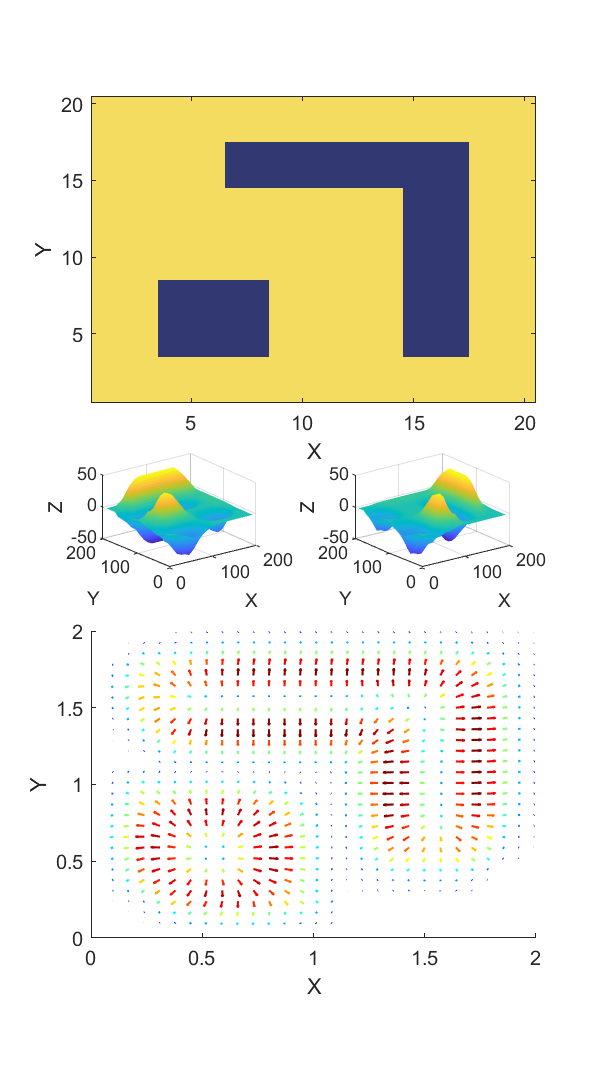
\includegraphics[width=1\linewidth]{demo-field1c.eps} % Replace 'example-image' with the filename of your image
	\caption{Visualization of the potential field calculated for the entire map using the proposed approach. Top: Obstacle distribution via a 2D heatmap. Center: Induced repulsive fields along X (left) and Y (right) axes. Bottom: Composite vector field showcasing the resultant repulsive velocities for obstacle avoidance.}
	\label{fig:example-field}
\end{figure}
%
%\add{add label, caption, every plot has different axis scale}
%
%\comment{}{we dont have the close obstacles bottlenecks, we do have weird bottlenecks in the orthagonal directions - maybe}
%
\subsection{Manipulator Examples}

%Delovanje potencialnega polja smo prikazali na dveh različnih primerih manipulatorja. Pri tem je ločljivost naše mreže voxlov ovir $R=10cm$. Uporaba interpolacije nam omogoča, da imamo relativno grobo mrežo voxlov, kar zniža spominsko zahtevnost mreže prostora, ter pospeši izračun. V primerih smo izbrali $K = 7$ POI točk interesa, v katerih gledamo oddaljenost od ovir, ki so enakomerno razporejene po segmentih in sklepih od drugega sklepa robota do vrha manipulatorja, torej od prve točke naprej, kjer se je manipulator sposoben izogniti oviri. POI so na grafih prikazani s pikami na manipulatorju. V bližini ovir iz njih segajo vektorji, ki prikazujejo izračunane odbojno hitrost v točkah. 

%Med izvajanjem simulacije izvajamo eulerjevo integracijo izračunanih sklepnih hitrosti, s korakom $T_{step}=0.1s$.

The operation of the potential field is demonstrated on two different manipulator cases. The resolution of our voxel grid for obstacles is \( R=10cm \). The use of interpolation allows us to have a relatively coarse voxel grid, which reduces the memory demand of the space grid and accelerates the computation. We selected \( K = 7 \) Points of Interest (POI) to observe the distance from obstacles and are uniformly distributed them along the segments and joints, starting from the second joint of the robot to the tip of the manipulator. This distribution begins from the second joint because it is from this point onwards that the manipulator has the capability to avoid obstacles. Points of Interest (POIs) are indicated by dots on the manipulator in the graphs. Near obstacles, vectors emanate from these points, depicting the calculated repulsive velocities at the locations. Throughout the simulation, Euler integration of the calculated joint velocities is performed with a step size of \( T_{step} = 0.1 \) s.

%V prvem primeru \ref{fig:keyframes-3d-column} manipulator z uporabo potencialnega polja izračunanega na predlagani način, se manipulator varno "zvije" oziroma izbere pot do točke, ki se nahaja na drugi strani stebra. Izbrane konstante primarne naloge so $k_v=5$ in $k_w=20$. Izbrane konstante obteženosti posameznih POI so $\alpha=\frac{\left[ \frac{3}{9}, \frac{2}{9}, \frac{1}{9}, \frac{1}{9}, \frac{1}{9}, \frac{1}{9}
% \right]}{10}$. Najkrajša pot vrha v točko pelje direktno skozi steber. Primarna naloga je, da vrh preide v želeno pozicijo in orientacijo. Ker je naloga vrha primarna, moramo uvesti znižanje primarne hitrosti v bližini ovire $\xi_{p}=1$, da ima sekundarna naloga dovolj prostosti in časa, da lahko izvede rekonfiguracijo za obhod stebra. Simulacijo izvajamo $50$ korakov. 

In the first case (Fig. \ref{fig:keyframes-3d-column}, \ref{fig:plots-3d-column}), the manipulator safely 'curls' or selects a path to a point located on the other side of a column, avoiding the obstacle with the potential field calculated by the proposed method. The constants chosen for the primary task are \( k_v = 5 \) and \( k_w = 1.5 \), for the avoidance task \(k_r=20\). The weighting constants for the individual POIs are \( \alpha = \frac{[ \frac{3}{9}, \frac{2}{9}, \frac{1}{9}, \frac{1}{9}, \frac{1}{9}, \frac{1}{9} ]}{10} \), where the biggest weight belongs to the point on the manipulator which is closest to the obstacle and so on. As the most direct path for the end-effector to the target passes straight through the column, an approach that would result in a collision, we implement a reduction of the primary speed in the vicinity of the obstacle, setting \( \xi_{p} = 1 \). The simulation is performed for 50 steps. 

\begin{figure}
	\centering
	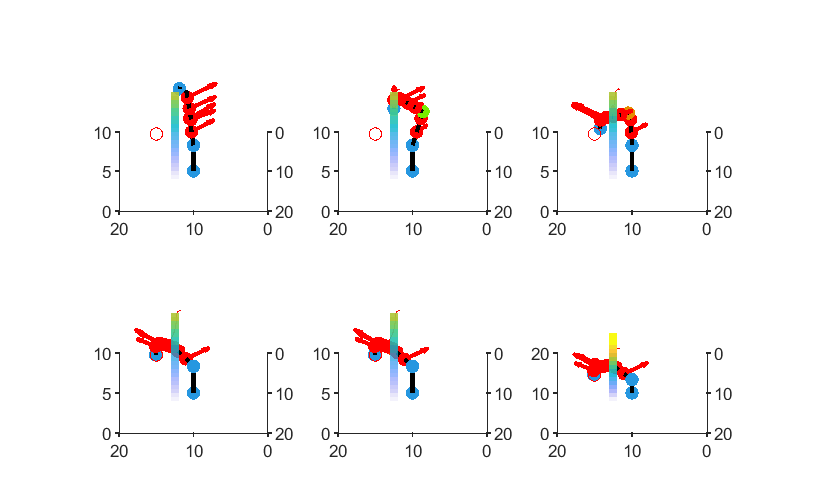
\includegraphics[width=1\linewidth]{keyframes_3D.eps} % Replace 'example-image' with the filename of your image
	\caption{Sequential keyframes demonstrating the manipulator's path planning and column obstacle avoidance strategy.}
	\label{fig:keyframes-3d-column}
\end{figure}


\begin{figure}
	\centering
	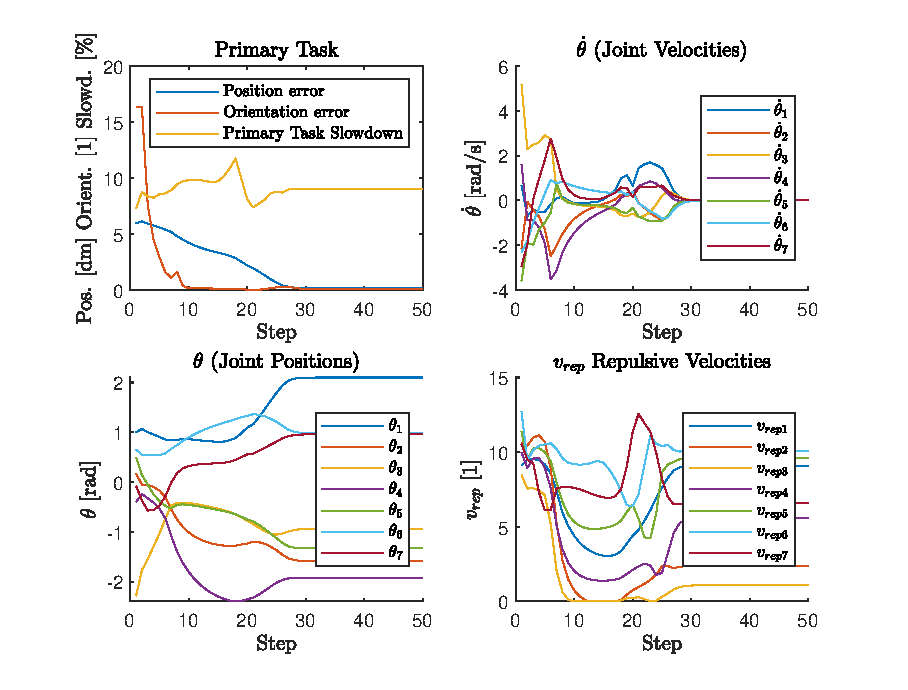
\includegraphics[width=1\linewidth]{4plots_column.eps} % Replace 'example-image' with the filename of your image
	\caption{Visualization of the manipulator's path around the column obstacle: (a) Primary Task errors and percentage of the primary speed after applying slowdown, (b) Joint Velocities $\dot{\theta}$, (c) Joint Positions $\theta$, and (d) Norms of Repulsive Velocities $v_{rep}$.}
	\label{fig:plots-3d-column}
\end{figure}

%V drugem primeru (Fig. \ref{fig:keyframes-3d-ball}, \ref{fig:plots-ball}) se naš robot giblje v dinamične okolju. Predlagan način izračuna odbojnih hitrosti je dobra izbira v primeru, ko potrebujemo lokalno optimizacijsko metodo za upoštevanje dinamičnih spremeb. V izbranem primeru imamo žogo, ki se med potekom optimizacije enakomerno premika iz leve strani grafa proti desni strani (torej v smeri y osi od 0.4 v trenutku 0 do 1.4 v zadnjem koraku simulacije). Primarna naloga ima sedaj nalogo vzdrževati vrh robota v eni točki, pri čemer smo za večjo sposobnost izogibanja oviri zanemarili izbiro orientacije vrha EE. To nam poveča sposobnost gibanja, posledično ne potrebujemo primary speed task slowdown  \( \xi_{p} = 0 \). The constants chosen for the primary task are \( k_v = 2 \) and \( k_w = 0 \), for the avoidance task \(k_r=3\). The weighting constants for the individual POIs are \( \alpha = \frac{[ \frac{1}{5}, \frac{1}{5}, \frac{1}{5}, \frac{1}{5}, \frac{1}{5}, \frac{1}{5} ]}{10} \). 

In the second scenario (Fig. \ref{fig:keyframes-3d-ball}, \ref{fig:plots-ball}), our robot operates within a dynamic environment. The proposed method for calculating repulsive velocities proves to be a suitable choice when a local optimization approach is needed to accommodate dynamic changes. In this scenario, a ball moves consistently from the left to the right side of the graph (i.e., along the y-axis from 0.4 at the initial moment to 1.4 in the final step of the simulation), as governed by the equation \( y_{\text{ball}} = 0.4 + (1.4 - 0.4) \times \frac{N_{\text{step}}}{75} \),  with \( x_{\text{ball}} = 1.25 \) and \( z_{\text{ball}} = 0.7 \). The primary task is now to maintain the robot's end-effector (EE) at a fixed point, disregarding EE orientation to enhance obstacle avoidance capability. This increases maneuverability, thereby eliminating the need for primary speed task slowdown (\( \xi_{p} = 0 \)). Constants selected for the primary task are \( k_v = 2 \) and \( k_w = 0 \), and for the avoidance task \( k_r = 3 \). Weighting constants for the individual POIs are \( \alpha = \frac{[ \frac{1}{5}, \frac{1}{5}, \frac{1}{5}, \frac{1}{5}, \frac{1}{5}, \frac{1}{5} ]}{10} \). The simulation is performed for 75 steps. 

%\begin{figure}
%	\centering
%	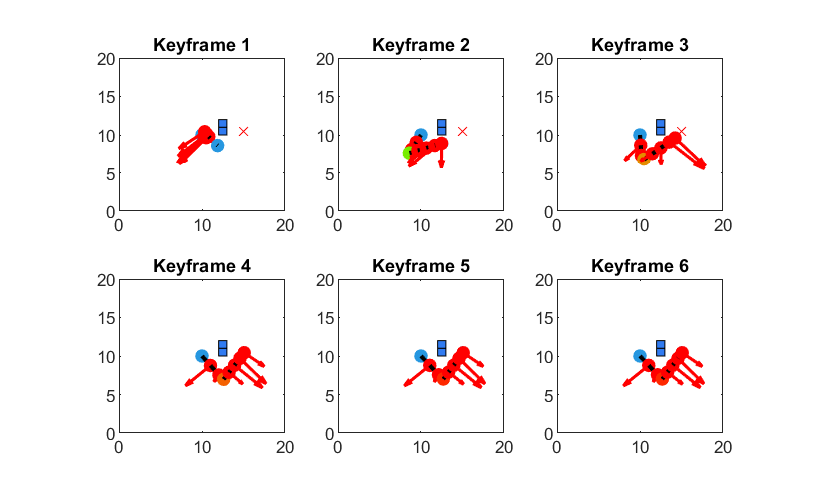
\includegraphics[width=1\linewidth]{keyframes_2D_a.eps} % Replace 'example-image' with the filename of your image
%	\caption{Example Image}
%	\label{fig:keyframes-2d-column}
%\end{figure}
%
%\begin{figure}
%	\centering
%	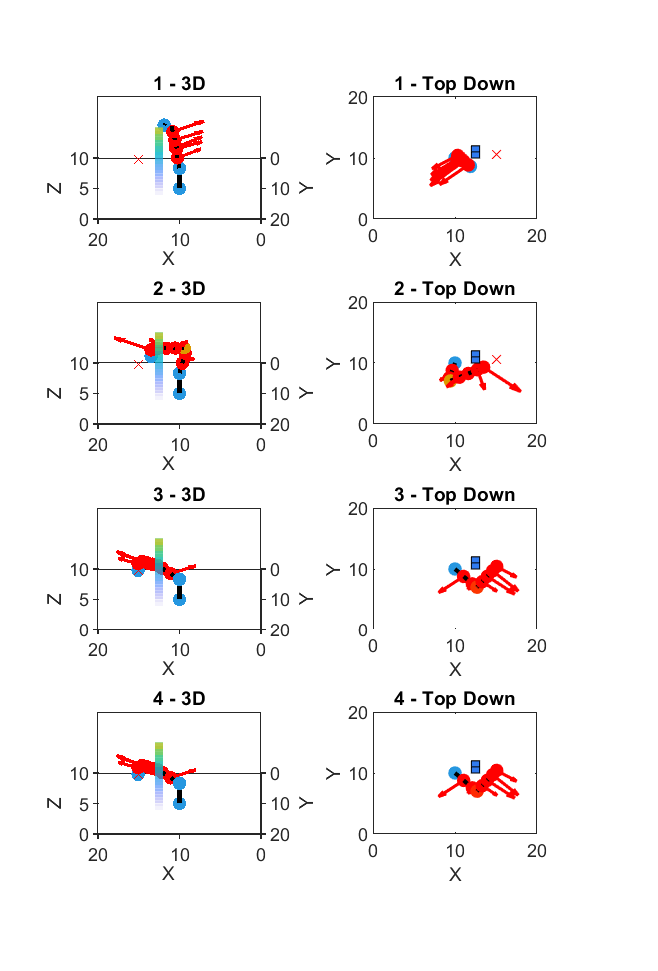
\includegraphics[width=1\linewidth]{keyframes_2_columns.eps} % Replace 'example-image' with the filename of your image
%	\caption{Example Image}
%	\label{fig:keyframes-2-column}
%\end{figure}
%
%
%\add{EXAMPLE: MANIPULATOR AND MOVING NOISY BALL}
%
\begin{figure}
	\centering
	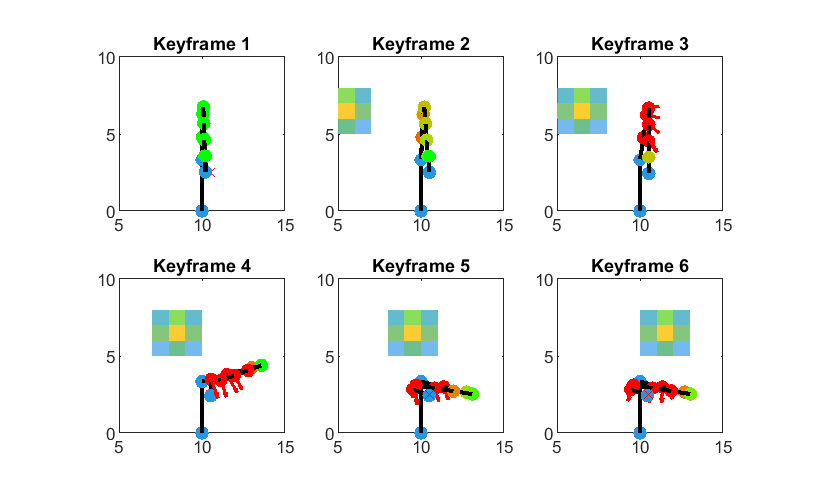
\includegraphics[width=1\linewidth]{keyframes_2D_ball.eps} % Replace 'example-image' with the filename of your image
	\caption{Dynamic obstacle avoidance scenario: Sequential keyframes illustrating the robot’s maneuvering in response to a progressively moving ball from left to right across the workspace.}
	\label{fig:keyframes-3d-ball}
\end{figure}
%
%\begin{figure}
%	\centering
%	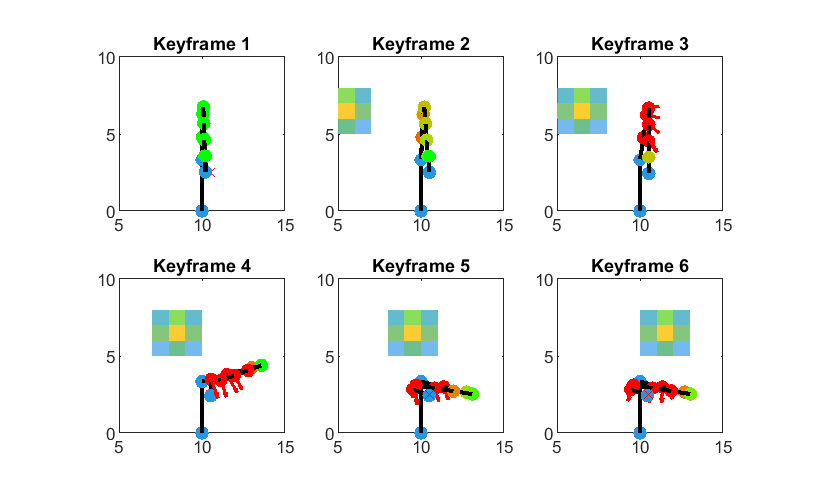
\includegraphics[width=1\linewidth]{keyframes_2D_ball.eps} % Replace 'example-image' with the filename of your image
%	\caption{Example Image}
%	\label{fig:keyframes-2d-ball}
%\end{figure}
%
\begin{figure}
	\centering
	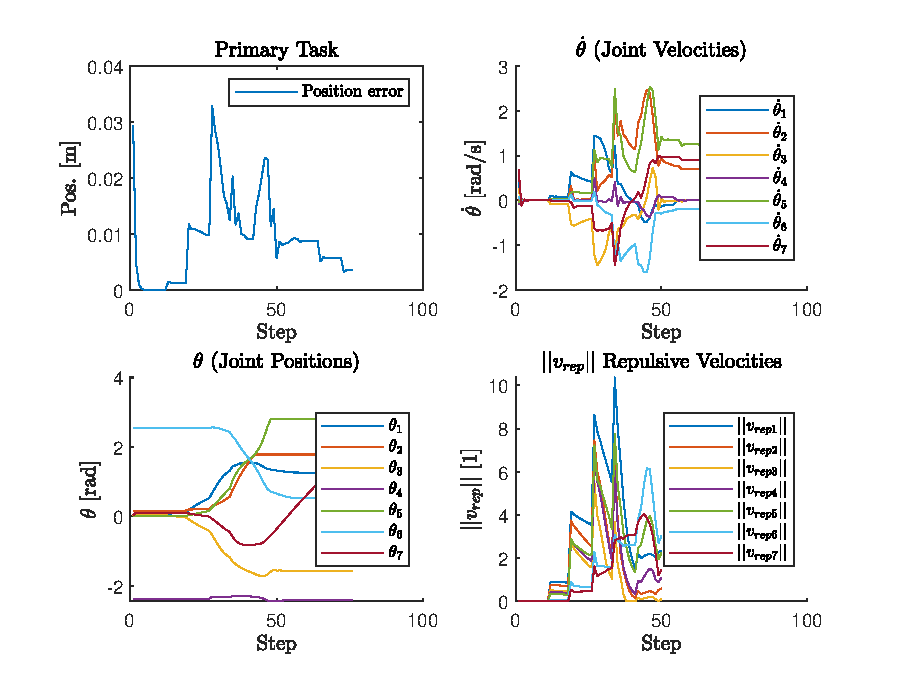
\includegraphics[width=1\linewidth]{4plots_ball.eps} % Replace 'example-image' with the filename of your image
	\caption{Performance in a dynamic obstacle avoidance scenario: (a) Primary Task error (b) Joint Velocities $\dot{\theta}$, (c) Joint Positions $\theta$, and (d) Norms of Repulsive Velocities $v_{rep}$.}
	\label{fig:plots-ball}
\end{figure}
%



\section{CONCLUSION}

\add{TODO}

\addtolength{\textheight}{-12cm}   % This command serves to balance the column lengths
                                  % on the last page of the document manually. It shortens
                                  % the textheight of the last page by a suitable amount.
                                  % This command does not take effect until the next page
                                  % so it should come on the page before the last. Make
                                  % sure that you do not shorten the textheight too much.


\begin{thebibliography}{99}
	
\bibitem{IDEASLab2023}
IDEAS Lab, "Motion and Path Planning," presented at Purdue University, 2023. [Online]. Available: \url{https://ideas.cs.purdue.edu/research/robotics/planning/}. Accessed on: Jan. 9, 2024.
	
\bibitem{c21} E. A. Basso and K. Y. Pettersen, “Task-Priority Control of Redundant Robotic Systems using Control Lyapunov and Control Barrier Function based Quadratic Programs,” in IFAC-PapersOnLine, vol. 53, no. 2, pp. 9037–9044, 2020. doi: 10.1016/j.ifacol.2020.12.2024.


\bibitem{c22} H. Toshani and M. Farrokhi, “Real-time inverse kinematics of redundant manipulators using neural networks and quadratic programming: A Lyapunov-based approach,” Robotics and Autonomous Systems, vol. 62, no. 6, pp. 766–781, Jun. 2014. doi: 10.1016/j.robot.2014.02.005.

\bibitem{haviland2021neo} J. Haviland and P. Corke, “NEO: A Novel Expeditious Optimisation Algorithm for Reactive Motion Control of Manipulators,” IEEE Robot. Autom. Lett., vol. 6, no. 2, Art. no. 2, Apr. 2021, doi: 10.1109/LRA.2021.3056060.


\bibitem{c23} Y. Zhang, S. S. Ge, and T. H. Lee, “A Unified Quadratic-Programming-Based Dynamical System Approach to Joint Torque Optimization of Physically Constrained Redundant Manipulators,” IEEE Trans. Syst., Man, Cybern. B, vol. 34, no. 5, pp. 2126–2132, Oct. 2004. doi: 10.1109/TSMCB.2004.830347.

\bibitem{c24} J. Nakanishi, R. Cory, M. Mistry, J. Peters, and S. Schaal, “Comparative experiments on task space control with redundancy resolution,” in Proc. 2005 IEEE/RSJ Int. Conf. on Intelligent Robots and Systems, Edmonton, Alta., Canada, 2005, pp. 3901–3908. doi: 10.1109/IROS.2005.1545203.

\bibitem{c25} M. H. Raibert and J. J. Craig, “Hybrid Position/Force Control of Manipulators,” Journal of Dynamic Systems, Measurement, and Control, vol. 103, no. 2, pp. 126–133, Jun. 1981. doi: 10.1115/1.3139652.

\bibitem{c26} T. Yoshikawa, “Dynamic hybrid position/force control of robot manipulators--Description of hand constraints and calculation of joint driving force,” IEEE J. Robot. Automat., vol. 3, no. 5, pp. 386–392, Oct. 1987. doi: 10.1109/JRA.1987.1087120.

\bibitem{c27} O. Khatib, “A unified approach for motion and force control of robot manipulators: The operational space formulation,” IEEE J. Robot. Automat., vol. 3, no. 1, pp. 43–53, Feb. 1987. doi: 10.1109/JRA.1987.1087068.

\bibitem{c28} N. Hogan, “Impedance Control: An Approach to Manipulation,” in Proc. 1984 American Control Conf., San Diego, CA, USA, Jul. 1984, pp. 304–313. doi: 10.23919/ACC.1984.4788393.

\bibitem{c29} A. A. Maciejewski and C. A. Klein, “Obstacle Avoidance for Kinematically Redundant Manipulators in Dynamically Varying Environments,” The International Journal of Robotics Research, vol. 4, no. 3, pp. 109–117, Sep. 1985. doi: 10.1177/027836498500400308.

\bibitem{c30} L. Lajpah and T. Petri, “Obstacle Avoidance for Redundant Manipulators as Control Problem,” in Serial and Parallel Robot Manipulators - Kinematics, Dynamics, Control and Optimization, S. Kucuk, Ed. InTech, 2012. doi: 10.5772/32651.

\bibitem{c31} R. Colbaugh and K. Glass, “Cartesian control of redundant robots,” J. Robotic Syst., vol. 6, no. 4, pp. 427–459, Aug. 1989. doi: 10.1002/rob.4620060409.

\bibitem{c32} K. Glass, R. Colbaugh, D. Lim, and H. Seraji, “Real-time collision avoidance for redundant manipulators,” IEEE Trans. Robot. Automat., vol. 11, no. 3, pp. 448–457, Jun. 1995. doi: 10.1109/70.388789.

\bibitem{c33} O. Khatib, “Real-time obstacle avoidance for manipulators and mobile robots,” in 1985 IEEE International Conference on Robotics and Automation Proceedings, Mar. 1985, pp. 500–505. doi: 10.1109/ROBOT.1985.1087247.

\bibitem{c34} L. Sciavicco and B. Siciliano, “A solution algorithm to the inverse kinematic problem for redundant manipulators,” IEEE J. Robot. Automat., vol. 4, no. 4, pp. 403–410, Aug. 1988. doi: 10.1109/56.804.

\bibitem{c35} L. Sciavicco and B. Siciliano, “Solving the Inverse Kinematic Problem for Robotic Manipulators,” in RoManSy 6, A. Morecki, G. Bianchi, and K. Kedzior, Eds., Boston, MA: Springer US, 1987, pp. 107–114. doi: 10.1007/978-1-4684-6915-8\_9.

\bibitem{c36} O. Egeland, “Task-space tracking with redundant manipulators,” IEEE J. Robot. Automat., vol. 3, no. 5, pp. 471–475, Oct. 1987. doi: 10.1109/JRA.1987.1087118.

\bibitem{c37} H. Seraji, “Configuration control of redundant manipulators: theory and implementation,” IEEE Trans. Robot. Automat., vol. 5, no. 4, pp. 472–490, Aug. 1989. doi: 10.1109/70.88062.

\bibitem{c38} Y. Nakamura, H. Hanafusa, and T. Yoshikawa, “Task-Priority Based Redundancy Control of Robot Manipulators,” The International Journal of Robotics Research, vol. 6, no. 2, pp. 3–15, Jun. 1987. doi: 10.1177/027836498700600201.

\bibitem{c39} B. Siciliano and O. Khatib, Eds., Springer Handbook of Robotics. in Springer Handbooks. Cham: Springer International Publishing, 2016. doi: 10.1007/978-3-319-32552-1.

\bibitem{c40} J.-O. Kim and P. Khosla, “Real-Time Obstacle Avoidance Using Harmonic Potential Functions,” 1992. doi: 10.1109/70.143352.

\bibitem{c41} L. Zlajpah and B. Nemec, “Kinematic control algorithms for on-line obstacle avoidance for redundant manipulators,” in Proc. IEEE/RSJ International Conference on Intelligent Robots and Systems, Lausanne, Switzerland, 2002, pp. 1898–1903. doi: 10.1109/IRDS.2002.1044033.

\bibitem{c42} T. Petrič and L. Žlajpah, “Smooth continuous transition between tasks on a kinematic control level: Obstacle avoidance as a control problem,” Robotics and Autonomous Systems, vol. 61, no. 9, Art. no. 9, Sep. 2013. doi: 10.1016/j.robot.2013.04.019.

\bibitem{c43} M. F. Pinto, T. R. F. Mendonça, L. R. Olivi, E. B. Costa, and A. L. M. Marcato, “Modified approach using variable charges to solve inherent limitations of potential fields method,” in Proc. 2014 11th IEEE/IAS International Conference on Industry Applications, Dec. 2014, pp. 1–6. doi: 10.1109/INDUSCON.2014.7059414.

\bibitem{c44} Z. Long, “Virtual target point-based obstacle-avoidance method for manipulator systems in a cluttered environment,” Engineering Optimization, vol. 52, no. 11, Art. no. 11, Nov. 2020. doi: 10.1080/0305215X.2019.1681986.

\bibitem{c45} A. H. Qureshi and Y. Ayaz, “Potential Functions based Sampling Heuristic For Optimal Path Planning,” Auton Robot, vol. 40, no. 6, Art. no. 6, Aug. 2016. doi: 10.1007/s10514-015-9518-0.

\bibitem{c46} A. H. Qureshi et al., “Adaptive Potential guided directional-RRT*,” in Proc. 2013 IEEE International Conference on Robotics and Biomimetics (ROBIO), Shenzhen, China, Dec. 2013, pp. 1887–1892. doi: 10.1109/ROBIO.2013.6739744.

\bibitem{c47} J. Yi, Q. Yuan, R. Sun, and H. Bai, “Path planning of a manipulator based on an improved P\_RRT* algorithm,” Complex Intell. Syst., vol. 8, no. 3, pp. 2227–2245, Jun. 2022. doi: 10.1007/s40747-021-00628-y.

\bibitem{c48} T. Zhu, J. Mao, L. Han, C. Zhang, and J. Yang, “Real-Time Dynamic Obstacle Avoidance for Robot Manipulators Based on Cascaded Nonlinear MPC With Artificial Potential Field,” IEEE Trans. Ind. Electron., pp. 1–11, 2023. doi: 10.1109/TIE.2023.3306405.

\bibitem{c49} X. Xia et al., “Path Planning for Obstacle Avoidance of Robot Arm Based on Improved Potential Field Method,” Sensors, vol. 23, no. 7, Art. no. 7, Apr. 2023. doi: 10.3390/s23073754.

\bibitem{c50} Y. Chen, L. Chen, J. Ding, and Y. Liu, “Research on Real-Time Obstacle Avoidance Motion Planning of Industrial Robotic Arm Based on Artificial Potential Field Method in Joint Space,” Applied Sciences, vol. 13, no. 12, p. 6973, Jan. 2023. doi: 10.3390/app13126973.

\bibitem{c51} S. M. LaValle, Planning Algorithms. Cambridge: Cambridge University Press, 2006.

\bibitem{c52} M. G. Tamizi, M. Yaghoubi, and H. Najjaran, “A review of recent trend in motion planning of industrial robots,” Int J Intell Robot Appl, vol. 7, no. 2, Art. no. 2, Jun. 2023. doi: 10.1007/s41315-023-00274-2.

\bibitem{vsvestka1997motion} P. {\v{S}}vestka and M. H. Overmars, “Motion planning for carlike robots using a probabilistic learning approach,” The International Journal of Robotics Research, vol. 16, no. 2, pp. 119–143, 1997.

\bibitem{lavalle1998rapidly} S. LaValle, “Rapidly-exploring random trees: A new tool for path planning,” Research Report 9811, 1998.

\bibitem{gammell2015batch} J. D. Gammell, S. S. Srinivasa, and T. D. Barfoot, “Batch Informed Trees (BIT*): Sampling-based Optimal Planning via the Heuristically Guided Search of Implicit Random Geometric Graphs,” in Proc. of the 2015 IEEE International Conference on Robotics and Automation (ICRA), May 2015, pp. 3067–3074. doi: 10.1109/ICRA.2015.7139620.

\bibitem{karaman2010incremental} S. Karaman and E. Frazzoli, "Incremental sampling-based algorithms for optimal motion planning," in Proc. Robotics: Science and Systems (RSS), 2010.

\bibitem{gammell2014informed} J. D. Gammell, S. S. Srinivasa, and T. D. Barfoot, “Informed RRT*: Optimal sampling-based path planning focused via direct sampling of an admissible ellipsoidal heuristic,” in Proc. of the 2014 IEEE/RSJ International Conference on Intelligent Robots and Systems, Chicago, IL, USA, Sep. 2014, pp. 2997–3004. doi: 10.1109/IROS.2014.6942976.

\bibitem{kuffner2000rrt} J. J. Kuffner and S. M. LaValle, “RRT-connect: An efficient approach to single-query path planning,” in Proceedings of the 2000 ICRA. Millennium Conference. IEEE International Conference on Robotics and Automation. Symposia Proceedings (Cat. No.00CH37065), Apr. 2000, pp. 995–1001 vol.2. doi: 10.1109/ROBOT.2000.844730.

\bibitem{siciliano1990kinematic} B. Siciliano, “Kinematic control of redundant robot manipulators: A tutorial,” J. Intell. Robot. Syst., vol. 3, no. 3, Art. no. 3, 1990, doi: 10.1007/BF00126069.

\bibitem{siciliano2016springer} B. Siciliano and O. Khatib, Eds., Springer Handbook of Robotics, in Springer Handbooks. Cham: Springer International Publishing, 2016. doi: 10.1007/978-3-319-32552-1.

\bibitem{siciliano2010robot} B. Siciliano, L. Sciavicco, L. Villani, and G. Oriolo, Robot. Model. Plan. Control, 2010, pp. 161–189. [Online]. Available: http://link.springer.com/10.1007/978-1-84628-642-1\_4

\bibitem{dai2022review} Y. Dai, C. Xiang, Y. Zhang, Y. Jiang, W. Qu, and Q. Zhang, “A Review of Spatial Robotic Arm Trajectory Planning,” Aerospace, vol. 9, p. 361, Jul. 2022, doi: 10.3390/aerospace9070361.

\bibitem{gottschalk1996obbtree} S. Gottschalk, M. C. Lin, and D. Manocha, “OBBTree: a hierarchical structure for rapid interference detection,” in Proceedings of the 23rd Annual Conference on Computer Graphics and Interactive Techniques, ACM, Aug. 1996, pp. 171–180. doi: 10.1145/237170.237244.

\bibitem{vandenbergen1997efficient} G. van den Bergen, “Efficient Collision Detection of Complex Deformable Models using AABB Trees,” Journal of Graphics Tools, vol. 2, no. 4, pp. 1–13, 1997. doi: 10.1080/10867651.1997.10487480.

\bibitem{chen2018path} G. Chen, D. Liu, Y. Wang, Q. Jia, and X. Zhang, “Path planning method with obstacle avoidance for manipulators in dynamic environment,” International Journal of Advanced Robotic Systems, vol. 15, no. 6, Art. no. 1729881418820223, Nov. 2018, doi: 10.1177/1729881418820223.

\bibitem{puiu2011realtime} D. Puiu and F. Moldoveanu, “Real-time collision avoidance for redundant manipulators,” in Proc. of the 2011 6th IEEE International Symposium on Applied Computational Intelligence and Informatics (SACI), Timisoara, Romania, 2011, pp. 403–408, doi: 10.1109/SACI.2011.5873037.

\bibitem{oleynikova2017voxblox} H. Oleynikova, Z. Taylor, M. Fehr, R. Siegwart, and J. Nieto, “Voxblox: Incremental 3D Euclidean Signed Distance Fields for on-board MAV planning,” in Proc. of the 2017 IEEE/RSJ International Conference on Intelligent Robots and Systems (IROS), Vancouver, BC, Sep. 2017, pp. 1366–1373. doi: 10.1109/IROS.2017.8202315.

\bibitem{wurmOctoMap} K. M. Wurm, A. Hornung, M. Bennewitz, C. Stachniss, and W. Burgard, “OctoMap: A Probabilistic, Flexible, and Compact 3D Map Representation for Robotic Systems,” [Details of publication, e.g., in Proc. of the Conference/Journal Name, Year, pp. Page numbers]. [DOI or URL if available].

\bibitem{gao2019flying} F. Gao, W. Wu, W. Gao, and S. Shen, “Flying on point clouds: Online trajectory generation and autonomous navigation for quadrotors in cluttered environments,” Journal of Field Robotics, vol. 36, no. 4, pp. 710–733, 2019, doi: 10.1002/rob.21842.

\bibitem{elfes1989using} A. Elfes, “Using occupancy grids for mobile robot perception and navigation,” Computer, vol. 22, no. 6, pp. 46–57, Jun. 1989, doi: 10.1109/2.30720.

\bibitem{han2019fiesta} L. Han, F. Gao, B. Zhou, and S. Shen, “FIESTA: Fast Incremental Euclidean Distance Fields for Online Motion Planning of Aerial Robots,” arXiv, Jul. 26, 2019. Accessed: Jan. 11, 2024. [Online]. Available: http://arxiv.org/abs/1903.02144

\bibitem{xu2021voxel} Y. Xu, X. Tong, and U. Stilla, “Voxel-based representation of 3D point clouds: Methods, applications, and its potential use in the construction industry,” Automation in Construction, vol. 126, p. 103675, Jun. 2021, doi: 10.1016/j.autcon.2021.103675.

\bibitem{niessner2013realtime} M. Nießner, M. Zollhöfer, S. Izadi, and M. Stamminger, “Real-time 3D reconstruction at scale using voxel hashing,” ACM Trans. Graph., vol. 32, no. 6, pp. 1–11, Nov. 2013, doi: 10.1145/2508363.2508374.

\bibitem{dryanovski2010multivolume} I. Dryanovski, W. Morris, and J. Xiao, “Multi-volume occupancy grids: An efficient probabilistic 3D mapping model for micro aerial vehicles,” in Proc. of the 2010 IEEE/RSJ International Conference on Intelligent Robots and Systems, Taipei, Oct. 2010, pp. 1553–1559. doi: 10.1109/IROS.2010.5652494.

\bibitem{thrun2002probabilistic} S. Thrun, Probabilistic robotics, vol. 45, 2002. Accessed: Jun. 14, 2023. [Online]. Available: https://dl.acm.org/doi/10.1145/504729.504754

\bibitem{lau2010improved} B. Lau, C. Sprunk, and W. Burgard, “Improved updating of Euclidean distance maps and Voronoi diagrams,” in Proc. of the 2010 IEEE/RSJ International Conference on Intelligent Robots and Systems, Taipei, Oct. 2010, pp. 281–286. doi: 10.1109/IROS.2010.5650794.

\bibitem{luo2018collisionfree} L. Luo et al., “Collision-Free Path-Planning for Six-DOF Serial Harvesting Robot Based on Energy Optimal and Artificial Potential Field,” Complexity, vol. 2018, pp. 1–12, Nov. 2018, doi: 10.1155/2018/3563846.

\bibitem{zhang2021obstacle} W. Zhang, H. Cheng, L. Hao, X. Li, M. Liu, and X. Gao, “An obstacle avoidance algorithm for robot manipulators based on decision-making force,” Robotics and Computer-Integrated Manufacturing, vol. 71, p. 102114, Oct. 2021, doi: 10.1016/j.rcim.2020.102114.

\bibitem{park2020trajectory} S.-O. Park, M. C. Lee, and J. Kim, “Trajectory Planning with Collision Avoidance for Redundant Robots Using Jacobian and Artificial Potential Field-based Real-time Inverse Kinematics,” Int. J. Control Autom. Syst., vol. 18, no. 8, Art. no. 8, Aug. 2020, doi: 10.1007/s12555-019-0076-7.

\bibitem{han2018dynamic} D. Han, H. Nie, J. Chen, and M. Chen, “Dynamic obstacle avoidance for manipulators using distance calculation and discrete detection,” Robotics and Computer-Integrated Manufacturing, vol. 49, pp. 98–104, Feb. 2018, doi: 10.1016/j.rcim.2017.05.013.

\bibitem{rong2006jump} G. Rong and T.-S. Tan, “Jump flooding in GPU with applications to Voronoi diagram and distance transform,” in Proceedings of the 2006 Symposium on Interactive 3D Graphics and Games - SI3D ’06, Redwood City, California, 2006, p. 109. doi: 10.1145/1111411.1111431.

\bibitem{szeliski2021computer} R. Szeliski, “Computer Vision: Algorithms and Applications, 2nd Edition,” Springer, 2021.

\bibitem{rosenfeld1968distance} A. Rosenfeld and J. L. Pfaltz, “Distance functions on digital pictures,” Pattern Recognition, vol. 1, no. 1, pp. 33–61, Jul. 1968, doi: 10.1016/0031-3203(68)90013-7.

\bibitem{felzenszwalb2012distance} P. F. Felzenszwalb and D. P. Huttenlocher, “Distance Transforms of Sampled Functions,” Theory of Comput., vol. 8, no. 1, pp. 415–428, 2012, doi: 10.4086/toc.2012.v008a019.

\bibitem{zhou2021egoplanner} X. Zhou, Z. Wang, H. Ye, C. Xu, and F. Gao, “EGO-Planner: An ESDF-Free Gradient-Based Local Planner for Quadrotors,” IEEE Robot. Autom. Lett., vol. 6, no. 2, pp. 478–485, Apr. 2021, doi: 10.1109/LRA.2020.3047728.

\bibitem{dryanovski2010multivolume} I. Dryanovski, W. Morris, and J. Xiao, “Multi-volume occupancy grids: An efficient probabilistic 3D mapping model for micro aerial vehicles,” in 2010 IEEE/RSJ International Conference on Intelligent Robots and Systems, Taipei: IEEE, Oct. 2010, pp. 1553–1559, doi: 10.1109/IROS.2010.5652494.



\end{thebibliography}




\end{document}
